% This file was created (at least in part) by the script ParseMdtoLatex by Louis du Plessis
% (Available from https://github.com/taming-the-beast)

\documentclass[11pt]{article}
%%%%%%%%%%%%%%%%%%%%%%%%%%%%%%%%%%%%%%%%%%%%%%%%%%%%%%%%%%%%%%%
% DO NOT EDIT THIS FILE UNLESS YOU KNOW WHAT YOU ARE DOING!!! %
%%%%%%%%%%%%%%%%%%%%%%%%%%%%%%%%%%%%%%%%%%%%%%%%%%%%%%%%%%%%%%%

% Useful packages
\usepackage[]{authblk}
\usepackage{graphicx}
\usepackage{color}
\usepackage{longtable}
\usepackage{hanging}
\usepackage{indentfirst}
\usepackage{setspace}
\usepackage{enumitem}
\usepackage{verbatim}
\usepackage{upgreek}
\usepackage{framed}
\usepackage{textcomp}
\usepackage{url}
\usepackage{soul}
\usepackage{amsmath,amsfonts,amssymb,mathrsfs}
\usepackage{fancyhdr}
\usepackage[compact]{titlesec}
\usepackage[T1]{fontenc}
\usepackage{lmodern}
\usepackage[utf8]{inputenc}
\usepackage[]{listings}
%\usepackage{fontspec}
\usepackage{placeins}
\usepackage{epstopdf}
\usepackage[export]{adjustbox}
\usepackage{tikz}
\usepackage[breaklinks]{hyperref}
\usepackage[all]{hypcap}


% References
\usepackage[backend=bibtex,hyperref=true,citestyle=authoryear,bibstyle=authortitle,firstinits=true,terseinits=true,doi=false,url=false,eprint=false,maxbibnames=10,maxcitenames=2]{biblatex}
\DeclareCiteCommand{\cite}
  {\usebibmacro{prenote}}
  {\usebibmacro{citeindex}%
   \printtext[bibhyperref]{\usebibmacro{cite}}}
  {\multicitedelim}
  {\usebibmacro{postnote}}

\DeclareCiteCommand*{\cite}
  {\usebibmacro{prenote}}
  {\usebibmacro{citeindex}%
   \printtext[bibhyperref]{\usebibmacro{citeyear}}}
  {\multicitedelim}
  {\usebibmacro{postnote}}

\DeclareCiteCommand{\parencite}[\mkbibparens]
  {\usebibmacro{prenote}}
  {\usebibmacro{citeindex}%
    \printtext[bibhyperref]{\usebibmacro{cite}}}
  {\multicitedelim}
  {\usebibmacro{postnote}}

\DeclareCiteCommand*{\parencite}[\mkbibparens]
  {\usebibmacro{prenote}}
  {\usebibmacro{citeindex}%
    \printtext[bibhyperref]{\usebibmacro{citeyear}}}
  {\multicitedelim}
  {\usebibmacro{postnote}}

\DeclareCiteCommand{\footcite}[\mkbibfootnote]
  {\usebibmacro{prenote}}
  {\usebibmacro{citeindex}%
  \printtext[bibhyperref]{ \usebibmacro{cite}}}
  {\multicitedelim}
  {\usebibmacro{postnote}}

\DeclareCiteCommand{\footcitetext}[\mkbibfootnotetext]
  {\usebibmacro{prenote}}
  {\usebibmacro{citeindex}%
   \printtext[bibhyperref]{\usebibmacro{cite}}}
  {\multicitedelim}
  {\usebibmacro{postnote}}

\DeclareCiteCommand{\textcite}
  {\boolfalse{cbx:parens}}
  {\usebibmacro{citeindex}%
   \printtext[bibhyperref]{\usebibmacro{textcite}}}
  {\ifbool{cbx:parens}
     {\bibcloseparen\global\boolfalse{cbx:parens}}
     {}%
   \multicitedelim}
  {\usebibmacro{textcite:postnote}}

\newcommand{\citep}{\parencite}
\newcommand{\citet}{\textcite}
\defbibheading{relevref}[\refname]{\section*{Relevant References}}

\renewcommand{\postnotedelim}{\iffieldpages{postnote}{\addcolon}{\addcomma\space}} 
\DeclareFieldFormat{postnote}{#1} 

\DeclareFieldFormat[article, inbook, incollection, inproceedings, patent, thesis, unpublished]{title}{#1}
\DeclareFieldFormat[article, inbook, incollection, inproceedings, patent, thesis, unpublished]{journaltitle}{\mkbibemph{#1}\nopunct}
\DeclareFieldFormat[article, inbook, incollection, inproceedings, patent, thesis, unpublished]{volume}{{#1}\addcolon} %puts volume number in parens
%\DeclareFieldFormat[article, inbook, incollection, inproceedings, patent, thesis, unpublished]{year}{\mkbibparens{#1}\nopunct} %puts year in parens

\DeclareFieldFormat[article, incollection, patent, thesis, unpublished]{pages}{{\nopp#1}}

\DeclareFieldFormat{sentencecase}{\MakeSentenceCase{#1}}

\renewbibmacro*{title}{%
  \ifthenelse{\iffieldundef{title}\AND\iffieldundef{subtitle}}
    {}
    {\ifthenelse{\ifentrytype{article}\OR\ifentrytype{inbook}%
      \OR\ifentrytype{incollection}\OR\ifentrytype{inproceedings}%
      \OR\ifentrytype{inreference}}
      {\printtext[title]{%
        \printfield[sentencecase]{title}%
        \setunit{\subtitlepunct}%
        \printfield[sentencecase]{subtitle}}}%
      {\printtext[title]{%
        \printfield[titlecase]{title}%
        \setunit{\subtitlepunct}%
        \printfield[titlecase]{subtitle}}}%
     \newunit}%
  \printfield{titleaddon}}

\DefineBibliographyStrings{english}{% various adjustments to common bib entry strings
urlseen = {Accessed:},% What goes in front of the date a URL was accessed/retrieved etc.
editor = {(Ed)},%Ed – no dot, in brackets
editors = {(Eds)},% Eds – no dot, in brackets
byeditor = {(Ed.)}}% ‘Edited by’ for edited works

\DeclareNameAlias{default}{last-first}

\renewbibmacro{in:}{}

\renewbibmacro{publisher+location+date}{
  \iflistundef{publisher}
    {}
    {\printlist{publisher}%
       {\addcomma\space}%
      \iflistundef{location}
        {}
        {\printlist{location}}%
    }
}

\DeclareBibliographyDriver{article}{%
\usebibmacro{bibindex}%
\usebibmacro{begentry}%
\usebibmacro{author/translator+others}%
\newunit\newblock
\printfield{year}%
\setunit{\labelnamepunct}\newblock
\usebibmacro{title}%
\newunit
\printlist{language}%
\newunit\newblock
\usebibmacro{byauthor}%
\newunit\newblock
\usebibmacro{bytranslator+others}%
\newunit\newblock
\printfield{version}%
\newunit\newblock
%\usebibmacro{in:}% %mit in:
\usebibmacro{journal}%
\newunit\newblock
\printfield{volume}%
\newunit\newblock
\usebibmacro{byeditor+others}%
\newunit\newblock
\usebibmacro{note+pages}%
\newunit\newblock
\iftoggle{bbx:isbn}
{}%
\newunit\newblock
\usebibmacro{doi+eprint+url}%
\newunit\newblock
\usebibmacro{addendum+pubstate}%
\newunit\newblock
\usebibmacro{pageref}%
\usebibmacro{finentry}}

\DeclareBibliographyDriver{inproceedings}{%
\usebibmacro{bibindex}%
\usebibmacro{begentry}%
\usebibmacro{author/translator+others}%
\newunit\newblock
\printfield{year}%
\setunit{\labelnamepunct}\newblock
\usebibmacro{title}%
\newunit
\printlist{language}%
\newunit\newblock
\usebibmacro{byauthor}%
\newunit\newblock
\usebibmacro{bytranslator+others}%
\newunit\newblock
\printfield{version}%
\newunit\newblock
%\usebibmacro{in:}% %mit in:
\usebibmacro{booktitle}%
\newunit\newblock
\printfield{volume}%
\newunit\newblock
\usebibmacro{byeditor+others}%
\newunit\newblock
\usebibmacro{publisher+location+date}%
\newunit\newblock
\usebibmacro{note+pages}%
\newunit\newblock
\usebibmacro{pageref}%
\usebibmacro{finentry}}

\DeclareBibliographyDriver{book}{%
\usebibmacro{bibindex}%
\usebibmacro{begentry}%
\usebibmacro{author/translator+others}%
\newunit\newblock
\printfield{year}%
\setunit{\labelnamepunct}\newblock
\usebibmacro{title}%
\newunit
\printlist{language}%
\newunit\newblock
\usebibmacro{byauthor}%
\newunit\newblock
\usebibmacro{bytranslator+others}%
\newunit\newblock
%\usebibmacro{in:}% %mit in:
\usebibmacro{booktitle}%
\newunit\newblock
\printfield{volume}%
\newunit\newblock
\usebibmacro{publisher+location+date}%
\newunit\newblock
\usebibmacro{note+pages}%
\newunit\newblock
\usebibmacro{pageref}%
\usebibmacro{finentry}}




% Page margins
\setlength{\evensidemargin}{0in}
\setlength{\headheight}{0in}
\setlength{\headsep}{0in}
\setlength{\oddsidemargin}{-0.25in}
\setlength{\paperheight}{11in}
\setlength{\paperwidth}{8.5in}
\setlength{\tabcolsep}{0in}
\setlength{\textheight}{9in}
\setlength{\textwidth}{7in}
\setlength{\topmargin}{0in}
\setlength{\topskip}{0in}
\setlength{\voffset}{0in}
\parskip = 0.15in
\pagestyle{plain}
\setlength{\parindent}{0cm}

% No white space between list items
\setlist{nolistsep}

% Hyperlink setup
\hypersetup{colorlinks=true,linkcolor=linkscol,citecolor=citescol,urlcolor=urlscol}

% Settings for code blocks
\lstset{backgroundcolor=\color[rgb]{0.972,0.972,0.972},
    tabsize=4,
    rulecolor=,
        basicstyle=\scriptsize,
        upquote=true,
        aboveskip={1.5\baselineskip},
        columns=fixed,
        showstringspaces=false,
        extendedchars=true,
        breaklines=true,
        prebreak = \raisebox{0ex}[0ex][0ex]{\ensuremath{\hookleftarrow}},
        frame=single,
        showtabs=false,
        showspaces=false,
        showstringspaces=false,
        identifierstyle=\ttfamily,
        keywordstyle=\color[rgb]{0,0,1},
        commentstyle=\color[rgb]{0.133,0.545,0.133},
        stringstyle=\color[rgb]{0.627,0.126,0.941}
}

% Colour definitions
\definecolor{citescol}{RGB}{194,101,1}
\definecolor{urlscol}{RGB}{0,150,206}
\definecolor{linkscol}{RGB}{149,0,207}
\definecolor{mycol}{RGB}{25,23,191}
\definecolor{outputcol}{RGB}{34,139,34}
\definecolor{tcol}{RGB}{165,0,14}







% TODO: The rest of the file needs to be cleaned up!
%       Past this point I am not sure what is necessary or not - Louis


\DeclareMathAlphabet{\msfsl}{T1}{cmr}{m}{it}
\DeclareMathAlphabet{\msyf}{OMX}{pcr}{m}{it}
\newcommand{\alf}{\upalpha}
\newcommand{\hilight}[1]{\colorbox{yellow}{#1}}

\newcommand{\levelone}[1]{
\bigskip
\noindent{\LARGE{\textsc{#1}}}
\vspace {0.05in}
}

\newcommand{\leveltwo}[1]{
\bigskip
\noindent{\Large{\textit{#1}}}
\vspace {-1mm}
}

\newcommand{\descriptionhead}[1]{
\noindent{\textcolor{mycol}{\textbf{\textit{#1}}}}\\ \vspace{-7mm}
}

\newcommand{\dhead}[1]{
\noindent{\textbf{\textit{#1 --}}}
}

\newcommand{\exs}[1]{
\vspace{-4mm}
\begin{itemize}
\item #1 \\ \vspace{-8mm}
\end{itemize}
}


\newcommand{\nbo}[1]{{\color{red}{#1}}}


\newcommand{\stepbullet}{\noindent \textbullet \ }
\newcommand{\mi}[1]{\textbf{\textit{#1}}}


\newcommand{\levelthree}[1]{\textit{#1 --}}


%\bibliographystyle{apalike}
%\bibpunct[; ]{(}{)}{;}{a}{,}{;}


\usepackage[breaklinks]{hyperref}
\usepackage[all]{hypcap}
\hypersetup{colorlinks=true,linkcolor=linkscol,citecolor=citescol,urlcolor=urlscol}

% Some macros for software packages
\newcommand{\R}{\texttt{R} }
\newcommand{\TESS}{\texttt{TESS}}
\newcommand{\PBD}{\texttt{PBD}}
\newcommand{\DDD}{\texttt{DDD}}
\newcommand{\Laser}{\texttt{laser}}
\newcommand{\TreePar}{\texttt{TreePar}}
\newcommand{\diversitree}{\texttt{diversitree}}
\newcommand{\RevBayes}{\texttt{RevBayes}}
\newcommand{\Rev}{\texttt{Rev}}
\newcommand{\MrBayes}{\texttt{MrBayes}}
\newcommand{\BEAST}{\texttt{BEAST}}
\newcommand{\PhyloBayes}{\texttt{PhyloBayes}}
\newcommand{\PAML}{\texttt{PAML}}

\let\otheriint\iint
\let\iint\relax
\usepackage{ wasysym }







\definecolor{shadecolor}{RGB}{194,225,255}

\setlength{\tabcolsep}{5pt}
\setlength{\topmargin}{-0.4in}
\setlength{\headheight}{14.5pt}
\pagestyle{fancy}

\newcommand{\taha}[1]{{\textcolor{red}{[TAH comment: #1]}}} % TAH comment

\titlespacing{\section}{0pt}{*0}{*0}
\titlespacing{\subsection}{0pt}{*0}{*0}
\titlespacing{\subsubsection}{0pt}{*0}{*0}

\titleformat{\section}
  {\normalfont\Large\bfseries\color{mycol}}
  {\thesection}{1em}{}

\titleformat{\subsection}
  {\normalfont\large\bfseries\color{mycol}}
  {\thesubsection}{1em}{}

\titleformat{\subsubsection}
  {\normalfont\bfseries\color{mycol}}
  {\thesubsubsection}{1em}{}

% command for MrBayes command-line step
\newcommand{\cl}[1]{{\texttt{\textbf{#1}}}}
\newcommand{\colx}[1]{{\textcolor{tcol}{#1}}}
\newcommand{\mbcl}[1]{\exs{\cl{MrBayes > {#1}}}}

\newcommand{\rbprmt}{RevBayes > } 
\newcommand{\rbcl}[1]{\exs{\cl{\rbprmt{#1}}}}
\newcommand{\rbout}[1]{\exs{\cl{\textcolor{outputcol}{#1}}}}
\newcommand{\rbdn}{{\Large \symbol{126}}} % This makes a copy/pasteable tilde
\newcommand{\rbclml}[1]{\exs{\cl{\ \ \ \ \ \ \ \ \ \ \ {#1}}}}

% text box settings
% requires compiling w/ XeLaTeX
%\newfontfamily\listingsfont[Scale=1.0]{Courier New}
%\lstset{basicstyle=\listingsfont, columns=texcl}
%\defaultfontfeatures{Mapping=tex-text}


\makeatletter
\lst@CCPutMacro\lst@ProcessOther {"2D}{\lst@ttfamily{-{}}{-{}}}
\@empty\z@\@empty
\makeatother



\setlength{\topmargin}{-0.4in}
\setlength{\headheight}{14.5pt}
\pagestyle{fancy}



\definecolor{lg}{gray}{0.75}
\def\gcirc{{%
    \setbox0\hbox{$\fullmoon$}%
    \rlap{\hbox to \wd0{\hss{$\textcolor{lg}{\newmoon}$}\hss}}\box0
}}



% Add your bibtex library here
\addbibresource{refs}


%%%%%%%%%%%%%%%%%%%%
% Do NOT edit this %
%%%%%%%%%%%%%%%%%%%%
\begin{document}
\renewcommand{\headrulewidth}{0.5pt}
\headsep = 20pt
\lhead{ }
\rhead{\textsc {BEAST v2 Tutorial}}
\thispagestyle{plain}


%%%%%%%%%%%%%%%%%%
% Tutorial title %
%%%%%%%%%%%%%%%%%%
\begin{center}

	% Enter the name of your tutorial here
	\textbf{\LARGE Tutorial using BEAST v2.4.7}\\\vspace{2mm}

	% Enter a short description of your tutorial here
	\textbf{\textcolor{mycol}{\Large Substitution-model-averaging}}\\

	\vspace{4mm}

	% Enter the names of all the authors here
	{\Large {\em David A. Rasmussen, Carsten Magnus and Remco Bouckaert}}
\end{center}



%%%%%%%%%%%%%%%%%
% Tutorial body %
%%%%%%%%%%%%%%%%%

\section{Background}\label{background}

Before running any phylogenetic analysis in BEAST, we need to decide on
a model of molecular evolution that describes how our sequence data
evolved. In particular, we need to decide on a substitution model that
describes the relative rates at which different types of substitutions
occur. For nucleotide data, the substitution model is typically
represented as a $4 \times 4$ symmetric rate matrix $ Q $ with the
general form:

\begin{equation}
    Q =
    \begin{pmatrix}
        - & r_{ac} & r_{ag} & r_{at} \\
        r_{ac} & - & r_{cg} & r_{ct} \\
        r_{ag} & r_{cg} & - & r_{gt} \\
        r_{at} & r_{ct} & r_{gt} & - \\
    \end{pmatrix}
\end{equation}

The different named substitution models (e.g.~JC69, HKY, TN93 and GTR)
group these rates into different categories. For example, the JC69 model
groups all rates together into a single rate category and assumes equal
equilibrium frequencies whereas the GTR model assigns each rate to a
different category and assumes a different equilibrium frequency for
each nucleotide. We are therefore faced with the difficult choice of
deciding \emph{a priori} which one of these substitution models is most
appropriate for our data.

\begin{framed}
\textbf{Topic for discussion:} In terms of phylogenetic inference, what
would the consequences be of picking a substitution model that is
overparameterized (too complex) for a given data set? What would the
consequences be of picking a model that is underparameterized?
\end{framed}

In addition to the substitution model, we also need to decide whether to
include rate heterogeneity across sites. We might also want to include a
proportion of invariant sites. On top of all this, we need to decide
whether to estimate nucleotide base frequencies or fix them at their
empirical frequencies. All of these choices leads to a bewildering
number of different models to choose from. For this reason, researchers
have often based their model choice on common conventions rather than on
which model is most appropriate for their data.

Fortunately, nowadays we can be more sophisticated in our modeling
choices and let the data inform us about which model is most appropriate
using Bayesian model averaging. In this tutorial, we will use BEAST2's
model averaging tool \textbf{bModelTest} \citep{Bouckaert2017} to select
the most appropriate substitution model for the primate mitochondrial
data set we already saw in the introductory tutorial.
\textbf{bModelTest} uses reversible jump MCMC (rjMCMC), which allows the
Markov chain to jump between states representing different possible
substitution models, much like we jump between different parameter
states in standard Bayesian MCMC inference. This allows us to treat the
substitution model as a nuisance parameter and integrate over all
\emph{available} (more on this later) substitution models while
simultaneously estimating the phylogeny and other model parameters.
Thus, parameter estimates are effectively averaged over different
substitution models, weighted by the support of each model. A useful
consequence is that as we are exploring the space of different
substitution models we also log the proportion of time that the Markov
chain spends in a particular model state. This can be interpreted as the
posterior support of a model, which tells us how strongly the data and
our prior beliefs support a model in comparison to other competing
models.

Note that \textbf{bModelTest} is only able to average over a subset of
substitution models that are (a) implemented in BEAST2 and (b) that it
knows how to move between. Ideally we would want to integrate over all
possible substitution models, but since non-reversible models are
mathematically inconvenient we restrict ourselves to the set of
time-reversible (symmetric) nucleotide substitution models, which leaves
us with 203 possible models. In addition, we can jump between models
with empirical/estimated base frequencies, with/without gamma
distributed rate heterogeneity and with/without invariant sites,
resulting in a total of $203 \times 2 \times 2 \times 2 = 1,624$ possible model
combinations. 

\section{Programs used in this
Exercise}\label{programs-used-in-this-exercise}

\subsubsection{BEAST2 - Bayesian Evolutionary Analysis Sampling
Trees}\label{beast2---bayesian-evolutionary-analysis-sampling-trees}

BEAST2 (\url{http://www.beast2.org}) is a free software package for
Bayesian evolutionary analysis of molecular sequences using MCMC and
strictly oriented toward inference using rooted, time-measured
phylogenetic trees. This tutorial is written for BEAST v2.4.7 \citep{Bouckaert2014}.

\subsubsection{BEAUti2 - Bayesian Evolutionary Analysis
Utility}\label{beauti2---bayesian-evolutionary-analysis-utility}

BEAUti2 is a graphical user interface tool for generating BEAST2 XML
configuration files.

Both BEAST2 and BEAUti2 are Java programs, which means that the exact
same code runs on all platforms. For us it simply means that the
interface will be the same on all platforms. The screenshots used in
this tutorial are taken on a Mac OS X computer; however, both programs
will have the same layout and functionality on both Windows and Linux.
BEAUti2 is provided as a part of the BEAST2 package so you do not need
to install it separately.

\subsubsection{Tracer}\label{tracer}

Tracer (\url{http://tree.bio.ed.ac.uk/software/tracer}) is used to
summarise the posterior estimates of the various parameters sampled by
the Markov Chain. This program can be used for visual inspection and to
assess convergence. It helps to quickly view median estimates and 95\%
highest posterior density intervals of the parameters, and calculates
the effective sample sizes (ESS) of parameters. It can also be used to
investigate potential parameter correlations. We will be using Tracer
v1.6.0.

\section{Practical: Selecting a substitution
model}\label{practical-selecting-a-substitution-model}

In this tutorial we will go through an analysis using bModelTest in
BEAST v2.4.7 and look into how to interpret the
results. This tutorial assumes that you have already done some of the
other tutorials and that you are familiar with the basics of using
BEAUti, BEAST and Tracer.

\subsection{Installing the bModelTest
Package}\label{installing-the-bmodeltest-package}

We first have to install the bModelTest (version 1.0.4 or above) package.

\begin{framed}
Open BEAUti and navigate to \textbf{File \textgreater{} Manage
Packages}. Select bModelTest and then click \textbf{Install/Upgrade}
(Figure \ref{fig:install}). Then \textbf{\emph{restart BEAUti}} to load
the package.
\end{framed}

\begin{figure}
    \centering
    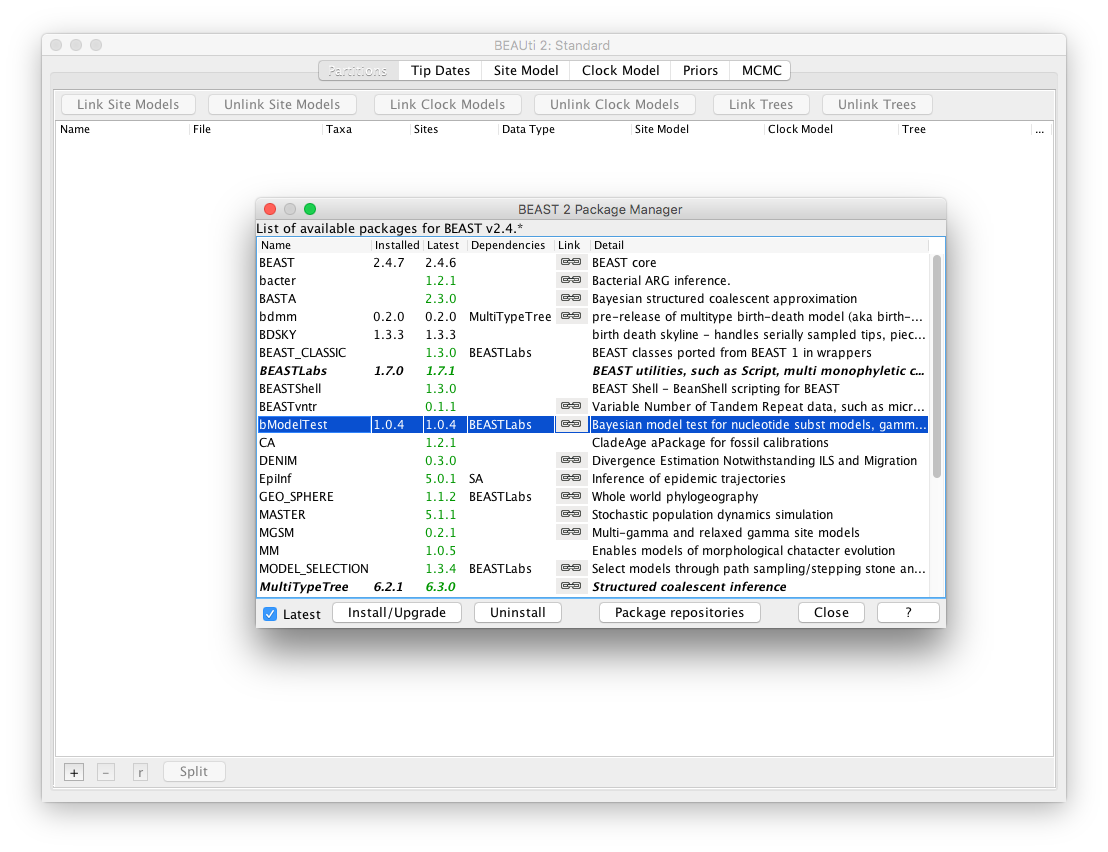
\includegraphics[width=0.800000\textwidth]{figures/install_bModelTest.png}
    \caption{Installing bModelTest in the Manage Packages window in BEAUti}
    \label{fig:install}
\end{figure}

\subsection{The Data}\label{the-data}

We will continue analyzing the primate mitochondrial data set from the
introductory tutorial.

\begin{framed}
Open BEAUti and navigate to \textbf{File \textgreater{} Import
Alignment}. Select the file \lstinline!primate-mtDNA.nex! in the data
directory.
\end{framed}

\subsection{Setting up the analysis in
BEAUti}\label{setting-up-the-analysis-in-beauti}

In this tutorial, we will simplify things by having all four partitions
in the alignment evolve under the same Site, Clock and Tree models.

\begin{framed}
In the \textbf{Partitions} panel select all four partitions (with
\textbf{shift+click}) and then click \textbf{Link Site Models},
\textbf{Link Clock Models} and \textbf{Link Trees}. You should rename
each model something more informative than noncoding, such as
\textbf{site}, \textbf{clock} and \textbf{tree}. Rename models by
\textbf{double-clicking} on the drop-down boxes.
\end{framed}

The Partition window should now look like Figure \ref{fig:partitions}.

\begin{figure}
    \centering
    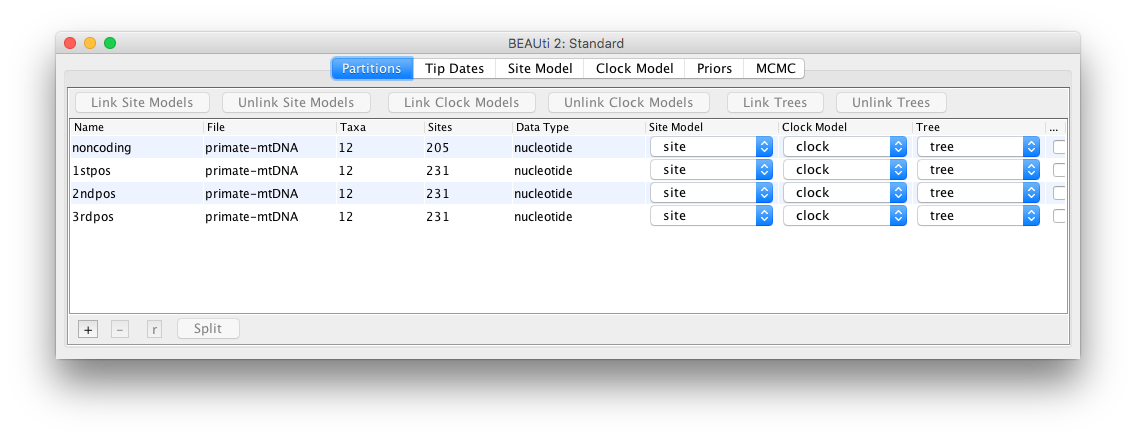
\includegraphics[max width=\textwidth, max height=0.9\textheight]{figures/partitions.png}
    \caption{Linking the Site Model across partitions in BEAUti.}
    \label{fig:partitions}
\end{figure}

Now we want to set up our Site Model to run the model averaging
analysis.

\begin{framed}
Click the \textbf{Site Model} tab in BEAUti and then select the
drop-down box at the top which says \textbf{Gamma Site Model} and change
it to \textbf{BEAST ModelTest} (Figure \ref{fig:siteModel}).
\end{framed}

\begin{figure}
    \centering
    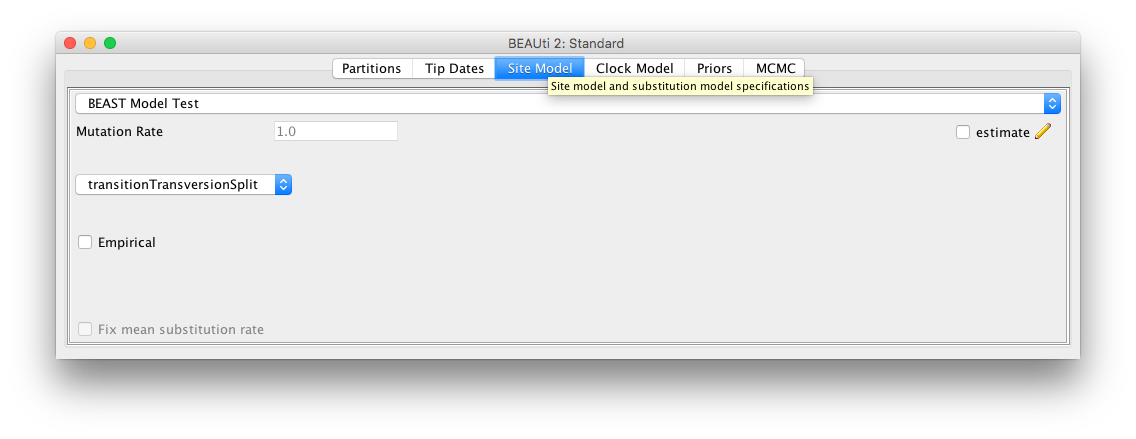
\includegraphics[max width=\textwidth, max height=0.9\textheight]{figures/siteModel.png}
    \caption{Setting up the BEAST ModelTest.}
    \label{fig:siteModel}
\end{figure}

In the lower drop-down box we will keep
\textbf{transitionTransversionSplit} selected. This tells bModelTest to
only consider substitution models that differentiate between transitions
(A $ \rightarrow $ G and C $ \rightarrow $ T)
and transversions (all other substitutions). Considering all the
different ways we can group the rates in the substitution matrix, there
are a total of 203 reversible models with symmetric matrices
\citep{Bouckaert2017}. However, if we only consider models that do not
group transitions together with transversions, there are only 31 models.
Selecting \textbf{transitionTransversionSplit} therefore dramatically
reduces the number of models that we need to explore.

In the \textbf{Clock Model} and \textbf{Prior} tabs, we do not need to
change any of the default settings for this tutorial.

\begin{framed}
Click the \textbf{MCMC} tab in BEAUti. Change the chain length to
5,000,000 and the sampling frequency to every 5,000. Change the
\textbf{tracelog} and \textbf{treelog} file names to
\lstinline!primate-mtDNA-bMT! and then click \textbf{File \textgreater{}
Save As} and save as \lstinline!primate-mtDNA-bMT.xml!.
\end{framed}

\subsection{Run the analysis in BEAST}\label{run-the-analysis-in-beast}

\begin{framed}
Open BEAST and choose \lstinline!primate-mtDNA-bMT.xml! as the BEAST XML
File (Figure \ref{fig:beastRun}). If BEAGLE is installed check the box
to use it. Then click \textbf{run}.
\end{framed}

\begin{figure}
    \centering
    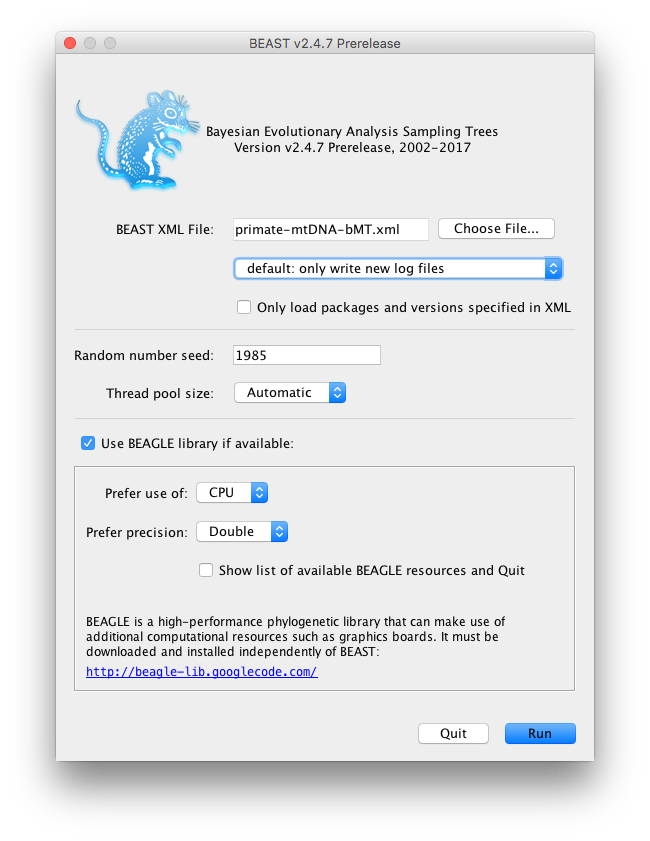
\includegraphics[width=0.500000\textwidth]{figures/beastRun.png}
    \caption{Running the analysis in BEAST.}
    \label{fig:beastRun}
\end{figure}

While BEAST is running consider the following discussion points.

We did not check \textbf{estimate} in the box next to the Mutation Rate
in the \textbf{Site Model} tab. Doing so makes no difference, since
BEAUti constrains the mean mutation rate of all partitions to be equal
to 1 (by default). Since we linked the substitution model across all
partitions we effectively have only one partition, thus the mutation
rate is fixed to 1.

Note that BEAUti (by default) does not allow us to estimate the clock
rate in the \textbf{Clock Model} tab. In this analysis we only have
contemporaneously sampled sequences and we did not set a calibration
node as in the introductory tutorial. Thus, we have no temporal
information and the clock rate is not uniquely identifiable. To make the
model identifiable BEAUti arbitrarily fixes the clock rate to 1.

\begin{framed}
\textbf{Topics for discussion:}

\begin{itemize}
\item
  We cannot estimate the substitution rate, so branches in the tree will
  not be measured in units of time. What will be the units for branch
  lengths in the estimated tree?
\item
  Suppose we used individual substitution models for each partition.
  What does the estimated mutation rate for each partition represent?
  Would the rate of each partition be identifiable?
\item
  What would happen if we removed the constraint to have a mean mutation
  rate of 1? What if we also added a calibration point?
\end{itemize}
\end{framed}

\subsection{Analyzing the output in
Tracer}\label{analyzing-the-output-in-tracer}

\begin{framed}
Open the \lstinline!primate-mtDNA-bMT.log! file in Tracer. There should
be a long list of entries in the window on the left hand side (Figure
\ref{fig:modelTrace}).
\end{framed}

If we select \textbf{BMT\_ModelIndicator} from the list of entries and
then \textbf{(I)nt} for the Data type below, we can see how the Markov
chain explored the space of different models by jumping between
substitution models. This is best seen if we click on the \textbf{Trace}
tab (Figure \ref{fig:modelTrace}). Here, the sampled integer values
refer to the indexes of the different substitution models. To see which
index corresponds to which model, refer to (Figure
\ref{fig:modelIndexes}).

Now click on the \textbf{Estimates} tab above. This frequency histogram
shows us how much time the Markov chain spent in each model state
relative to other model states, and therefore reflects the posterior
support for each model. We can see that the chain spent the most time in
model number 1 (Figure \ref{fig:modelPosterior}), which by consulting
Figure \ref{fig:modelIndexes} we see corresponds to the HKY model.

\begin{figure}
    \centering
    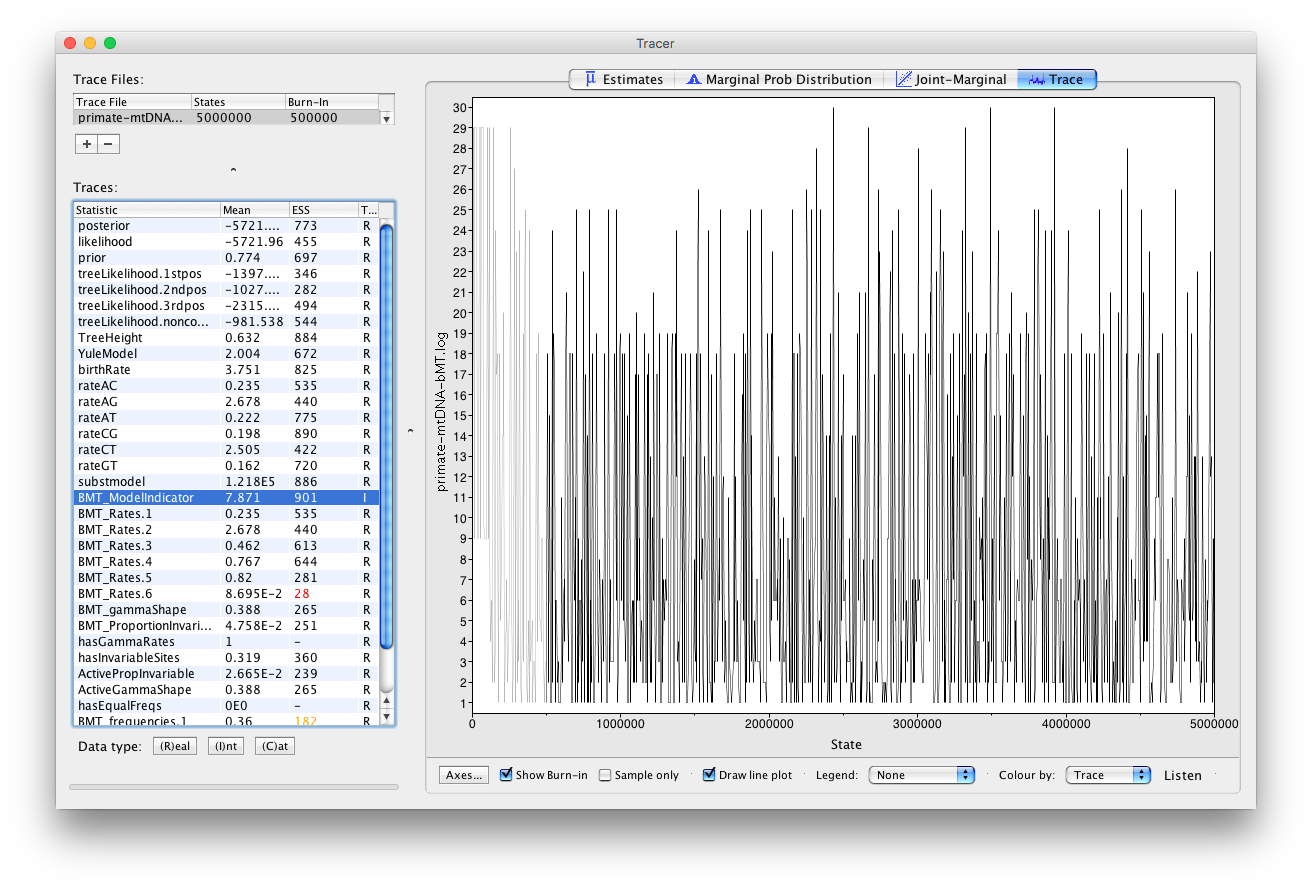
\includegraphics[width=0.800000\textwidth]{figures/modelTrace.png}
    \caption{Visualizing how the Markov chain explored different models in Tracer.}
    \label{fig:modelTrace}
\end{figure}

\begin{figure}
    \centering
    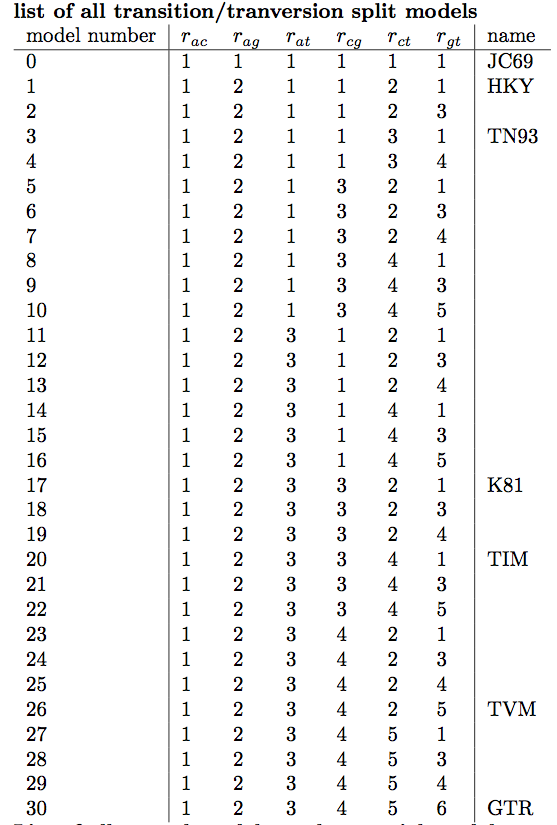
\includegraphics[width=0.500000\textwidth]{figures/modelIndexes.png}
    \caption{A list of substitution models, their associated model number (index) and how the substitution rates are grouped.}
    \label{fig:modelIndexes}
\end{figure}

\begin{figure}
    \centering
    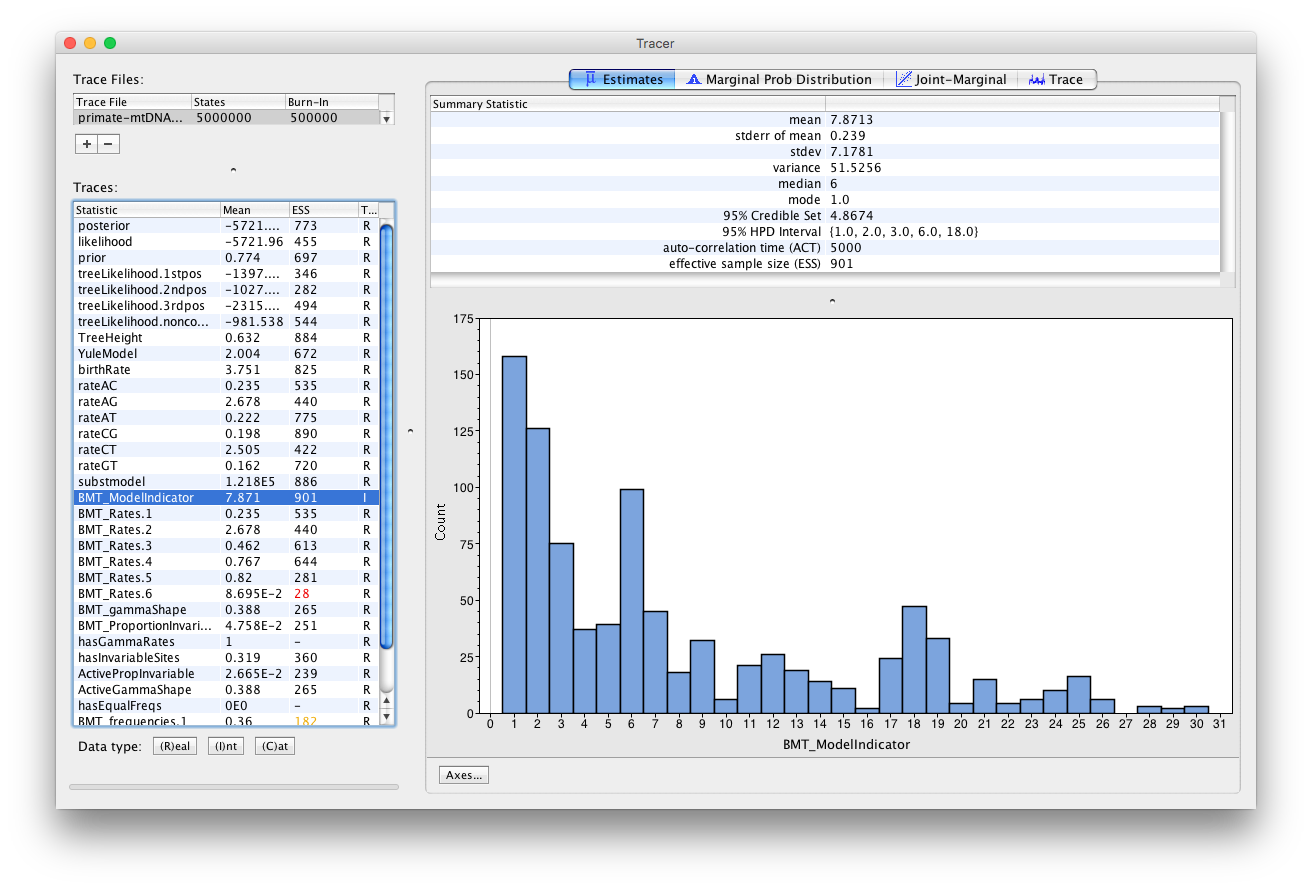
\includegraphics[width=0.800000\textwidth]{figures/modelPosterior.png}
    \caption{Visualizing the posterior support for different substitution models in Tracer.}
    \label{fig:modelPosterior}
\end{figure}

\begin{framed}
\textbf{Topic for discussion:} Did the chain ever visit the JC69 model?
Why not?
\end{framed}

We can also use the output of our analysis to see if a model with
(gamma) rate heterogeneity and/or a proportion of invariant sites is
supported. If we select \textbf{hasGammaRates} in the window on the left
and then click \textbf{Estimates} we see the proportion of time the
chain spent in a model state with rate heterogeneity on (1) versus off
(0), and thus the posterior support for a model with rate heterogeneity.
Here, the chain seems to remain in a state with rate heterogeneity on,
indicating very strong support for heterogeneity (Figure
\ref{fig:hasGammaRates}). We can also select \textbf{hasInvariableSites}
to see if a model with invariant sites is supported. Here we see that
the model spends more time in a model state with invariant sites off (0)
than on (1), indicating that the presence of invariant sites are not as
strongly supported important (Figure \ref{fig:hasInvariableSites}). Note
that we can also look at the traces for \textbf{BMT\_gammaShape} and
\textbf{BMT\_ProportionInvariant} to see which values of these two
parameters the chain visited.

There are a few other things we can look at in Tracer as well:

\begin{itemize}

\item
  \textbf{rateAC, \ldots{} ,rateGT} are the substitution rates between
  pairs of nucleotides in the substitution matrix. Note that these rates
  are averaged over all the models, weighted by the time the Markov
  chain spent in each model state.
\item
  \textbf{BMT\_Rates.1 to 6} are the independent substitution rates used
  to build up the rate matrix. They are indexed by how they are grouped
  into the six different possible rate categories (see Figure
  \ref{fig:modelIndexes}). Note that not all the models averaged over
  use all 6 independent rate parameters.
\item
  \textbf{ActiveGammaShape/PropInvariable} are the gamma shape parameter
  and the proportion of variables sites when active, that is, when
  \textbf{hasGammaRates} and \textbf{hasInvariableSites} are selected.
  To get the estimate of the mean of the shape parameter, divide the
  mean \textbf{ActiveGammaShape} by the mean of \textbf{hasGammaRates}.
\item
  \textbf{hasEqualFreqs} indicates if the chain is in a state with equal
  nucleotide base frequencies.
\end{itemize}

\begin{figure}
    \centering
    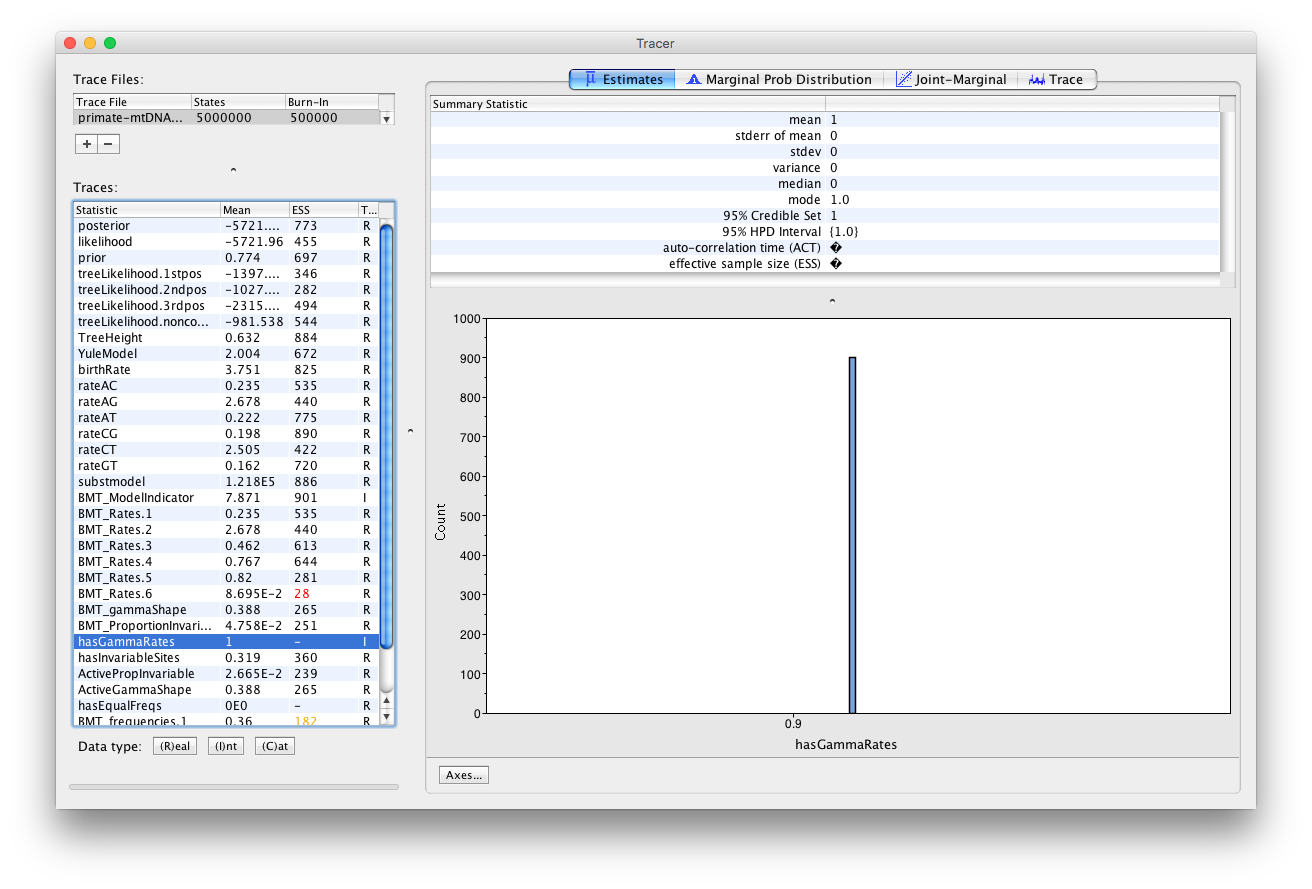
\includegraphics[width=0.800000\textwidth]{figures/hasGammaRates.png}
    \caption{The posterior support for including gamma rate heterogeneity.}
    \label{fig:hasGammaRates}
\end{figure}

\begin{figure}
    \centering
    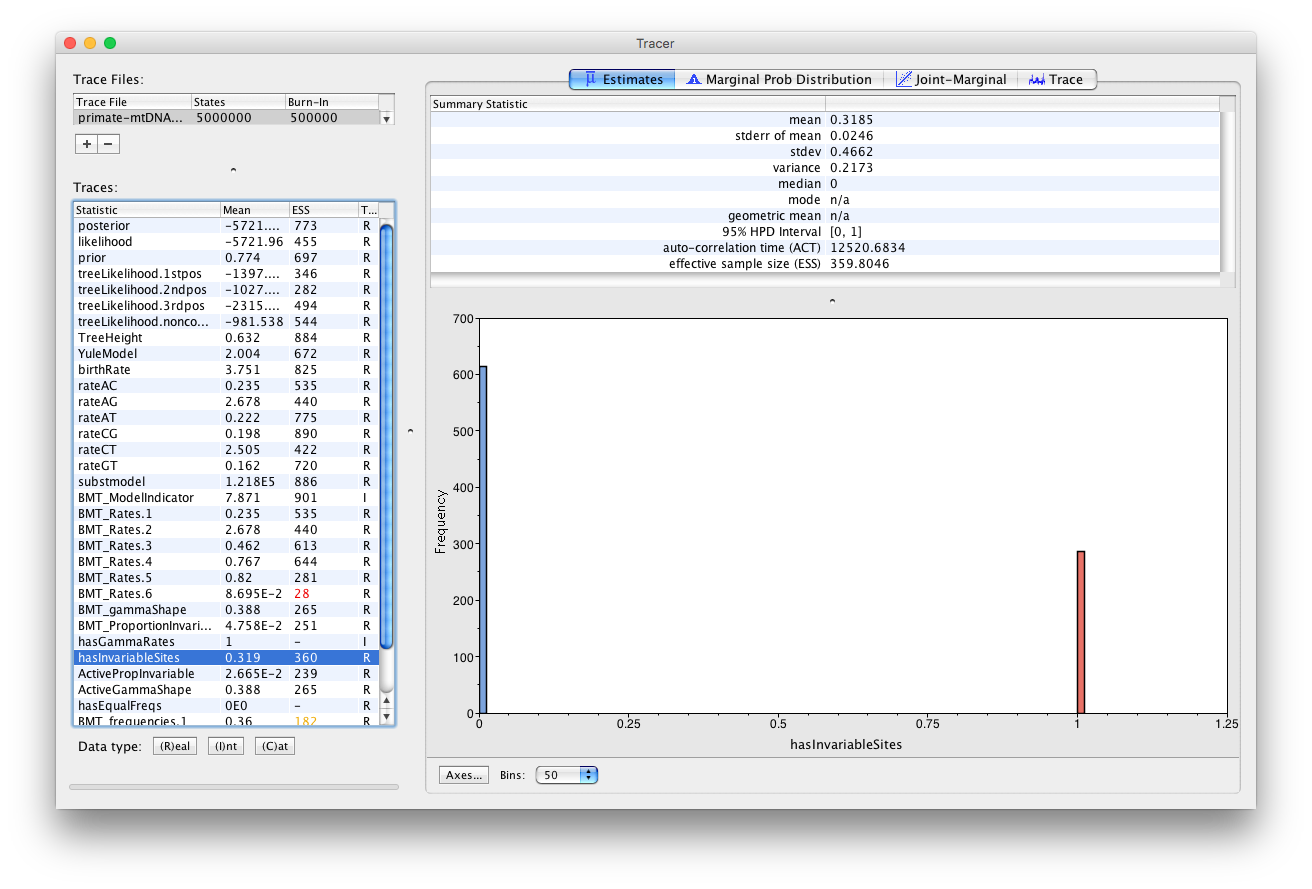
\includegraphics[width=0.800000\textwidth]{figures/hasInvariableSites.png}
    \caption{The posterior support for including a proportion of invariant sites.}
    \label{fig:hasInvariableSites}
\end{figure}

\begin{framed}
\textbf{Topic for discussion:} Why does \textbf{BMT\_Rates.6} not mix
poorly?

\textbf{Hint:} Look at the table of substitution models and the
distribution and trace of \textbf{BMT\_ModelIndicator} in Tracer.

\textbf{Bonus hint:} Look at the trace for \textbf{BMT\_Rates.6} and
plot the joint-marginal between \textbf{BMT\_Rates.1} and
\textbf{BMT\_Rates.2}.
\end{framed}

Select pairs of the \textbf{rateAC, \ldots{} ,rateGT} parameters (using
\textbf{shift+click}) and click on the \textbf{Joint-Marginal} tab to
investigate parameter correlations (Figure \ref{fig:rateCorrelations}).
Try looking at \textbf{rateAT} vs. \textbf{rateCG} and \textbf{rateCG}
vs \textbf{rateGT}).

\begin{figure}
    \centering
    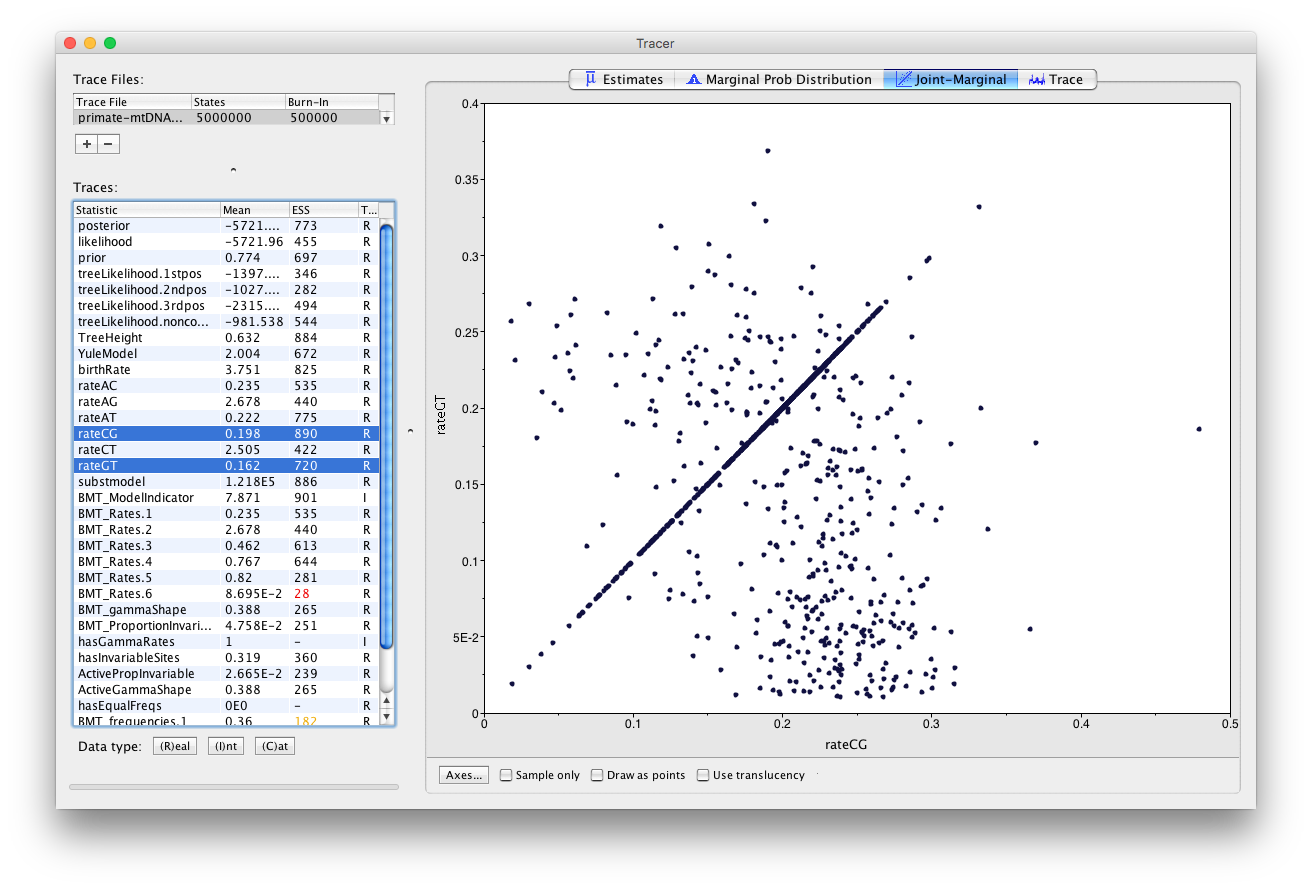
\includegraphics[width=0.800000\textwidth]{figures/rateCorrelations.png}
    \caption{Correlations between rate parameters.}
    \label{fig:rateCorrelations}
\end{figure}

\begin{framed}
\textbf{Topic for discussion:} It appears that some pairs of the rate
parameters are highly correlated for some samples and uncorrelated for
the rest. What is happening here? Should we be worried about these
parameter correlations?

Do you also see correlations between the \textbf{BMT\_Rates.1 to 6}
parameters?
\end{framed}

\subsection{Analyzing the output using
BModelAnalyzer}\label{analyzing-the-output-using-bmodelanalyzer}

Another really nice feature of bModelTest is that we can graphically
analyze the output using the \textbf{BModelAnalyser App}.

\begin{framed}
In BEAUti, select \textbf{File \textgreater{} Launch Apps} and then
launch the \textbf{BModelAnalyser App}. A dialogue window should pop up
(Figure \ref{fig:analyzerDialogue}). Enter
\lstinline!primate-mtDNA-bMT.log! as the file to analyze. You can leave
the other entries at their default settings but make sure
\textbf{transitionTransversionSplit} is selected for the Model Set and
the box next to \textbf{Use Browser For Visualization} is checked. Then
click \textbf{OK}.
\end{framed}

\begin{figure}
    \centering
    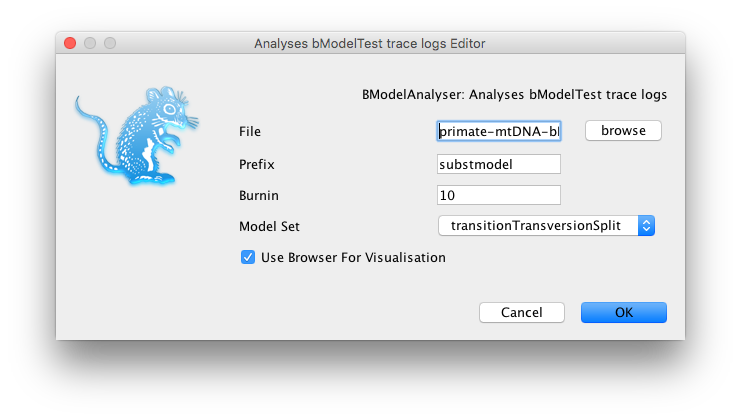
\includegraphics[width=0.600000\textwidth]{figures/analyzerDialogue.png}
    \caption{Running the BModelAnalyser App.}
    \label{fig:analyzerDialogue}
\end{figure}

After BModelAnalyser runs, a new window should appear in your default
web browser that represents the model selection results graphically
(Figure \ref{fig:modelGraph}). This graph depicts the nested
relationship of the different substitution models: an arrow pointing
from one model to another indicates that the model at the tail is nested
within the model at the head of the arrow. As we can see, JC69 is nested
within all other models and all other models are nested within GTR.

\begin{figure}
    \centering
    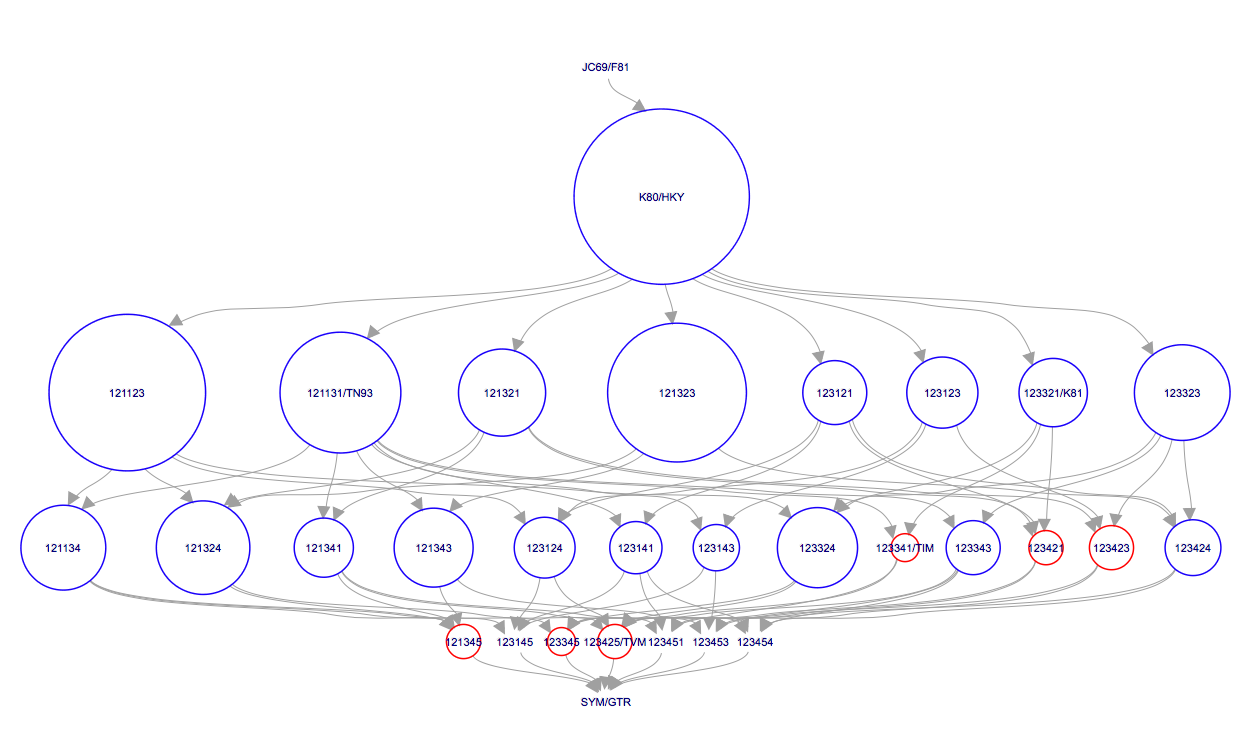
\includegraphics[max width=\textwidth, max height=0.9\textheight]{figures/modelGraph2.png}
    \caption{A graphical representation of the model selection results produced by BModelAnalyzer.}
    \label{fig:modelGraph}
\end{figure}

The area of the circle surrounding each model is proportional to the the
posterior support for that model. The colours represent whether the
model is contained within the 95\% credible set (blue) or not (red). For
the primate data set, the HKY model clearly has the highest posterior
support (Figure \ref{fig:modelGraph}). However, other models such as
TN93 and two unnamed models, \textbf{121323} and \textbf{121123}, also
have fairly high posterior support. The six digit model code describes
how the different substitution rates are grouped in the order of
$ r_{ac} $, $ r_{ag} $, $ r_{at} $,
$ r_{cg} $, $ r_{ct} $ and
$ r_{gt} $. For instance, \textbf{121323} is a slight
variant of the HKY model with an additional group for the rates
$ r_{ct} $ and $ r_{gt} $. The six digit codes
for all models are shown in Figure \ref{fig:modelIndexes}.

\begin{framed}
\textbf{Topic for discussion:} We have used bModelTest to explore a
large set of substitution models. But how do we know that any of the
substitution models actually fit the observed sequence data well?
\end{framed}

\section{Acknowledgment}\label{acknowledgment}

This tutorial is based on the original bModelTest tutorial by Remco
Bouckaert.

\section{Useful Links}\label{useful-links}

\begin{itemize}

\item
  Official bModelTest documentation:
  \url{https://github.com/BEAST2-Dev/bModelTest/wiki}
\item
  The original bModelTest tutorial is available here:
  \url{https://github.com/BEAST2-Dev/bModelTest/releases/download/v0.3.0/bModelTestTutorial.pdf}
  and is also included in the source code. 
\end{itemize}



%%%%%%%%%%%%%%%%%%%%%%%
% Tutorial disclaimer %
%%%%%%%%%%%%%%%%%%%%%%%
% Please do not change the license
% Add the author names and relevant links
% Add any other aknowledgments here
\href{http://creativecommons.org/licenses/by/4.0/}{
\includegraphics[scale=0.8]{figures/ccby.pdf}} This tutorial was written by David A. Rasmussen, Carsten Magnus and Remco Bouckaert for \href{https://taming-the-beast.github.io}{Taming the BEAST} and is licensed under a \href{http://creativecommons.org/licenses/by/4.0/}{Creative Commons Attribution 4.0 International License}. 


%%%%%%%%%%%%%%%%%%%%
% Do NOT edit this %
%%%%%%%%%%%%%%%%%%%%
Version dated: \today




%%%%%%%%%%%%%%%%
%  REFERENCES  %
%%%%%%%%%%%%%%%%

\printbibliography[heading=relevref]


\end{document}